

% The following makes latex use nicer postscript fonts.

\documentclass[a4paper,10pt]{report}

\usepackage[a4paper]{geometry}
\usepackage[dutch]{babel}
\usepackage{lmodern}
\usepackage{amssymb,amsmath}
\usepackage[T1]{fontenc}
%\usepackage[utf8]{inputenc}
\usepackage{microtype}
\usepackage{longtable,booktabs}
\usepackage[unicode=true]{hyperref}
\usepackage{graphicx}
\usepackage[space]{grffile}
\usepackage{lscape}
\usepackage{listings}
\usepackage{tabularx}
\usepackage{vubtitlepage}
\usepackage{tikz,pgfplots}
\usepackage{mathtools}
\usepackage{caption}
\usepackage{apacite}
\usepackage{subfig}
\usepackage{siunitx}
\usepackage{pgfplots} 
\usepackage{pgfplotstable}
\usepackage[round]{natbib}
\usepackage[toc,page]{appendix}
\usepackage{xr}
\usepackage{adjustbox}
\externaldocument{sections/lectuur}
\externaldocument{sections/experiment}
\newcommand{\argmax}[1]{\underset{#1}{\operatorname{arg}\,\operatorname{max}}\;}
\usepackage{array}
\usepackage{multirow}
\usepackage{tabu}

\newcommand\MyBox[2]{
  \fbox{\lower0.75cm
    \vbox to 1.7cm{\vfil
      \hbox to 1.7cm{\hfil\parbox{1.4cm}{#1\\#2}\hfil}
      \vfil}%
  }%
}
\setlength{\parindent}{0em}

\author{Yannick Merckx}
\title{Gevoelsanalyse in het Nederlands}

\promotortitle{Promotor}
\promotor{Yann-Micha\"el De Hauwere}
\advisors{Maarten Deville\\
          Peter Vrancx}
\advisortitle{Begeleiders}
\faculty{Faculteit Wetenschappen}
\department{Departement Computerwetenschappen}
\reason{Bachelorproef}
\date{Juni 2015}
\rolenumber{Rolnummer: 500294}
          
\begin{document}

% First dutch TitlePage
\maketitlepage

\setlength{\arrayrulewidth}{0.1mm}

\newpage

\begin{abstract}
Gevoelsanalyse is een populaire gegeven binnen de Machine Learning. In deze bachelorproef gaan we op zoek of het mogelijk is om aan de hand van enkele eenvoudige machine learning technieken een gevoelsanalyse uit te voeren. Specifieker focussen we op de Nederlandse taal, waar het naslagwerk vandaag de dag eerder beperkt van is. Als onderwerp van de gevoelsanalyse worden film-,boek- en muziekrecensies aan de hand van een algoritme beoordeeld of ze een positieve of negatieve emotie uitdrukken. Voor het onderzoek bekijken we de theoretische kant van een gevoelsanalyse, waar we de mogelijke technieken bespreken. Daarnaast wordt ook de praktische zijde uitgewerkt waar we de theoretische kennis gaan omzetten in een experiment. Dit experiment toont aan dat het mogelijk is om gevoelsanalyse uit te voeren op het Nederlands.
\end{abstract}

\renewcommand{\abstractname}{Dank woord}
\begin{abstract}
Het maken van een bachelorproef doe je nooit alleen, daarom ook een woord van dank aan enkele mensen waarop ik gedurende mijn eindwerkproces steeds kon terugvallen. Als eerste zou ik graag mijn begeleiders, Maarten Deville en Peter Vranckx, van harte willen bedanken voor hun grote steun en inzet gedurende het hele jaar. Ze waren gedurende het hele jaar altijd beschikbaar om op al mijn vragen een snel antwoord te geven. Als laatste wens ik ook mijn dank uit te drukken aan mijn promotor, Yann-Micha\"el De Hauwere. Bij de korte evaluaties was hij altijd aanwezig en stond hij mij altijd bij voor raad en daad.
\end{abstract}
\renewcommand{\contentsname}{Inhoud}
\tableofcontents
\include{sections/introductie}


\chapter{Achtergrondinformatie}\label{Achtergrondinformatie}

In dit hoofdstuk bespreken we de technieken, classifiers en de valkuilen voor het onderzoek, waar zeker rekening mee moet gehouden worden. Zoals eerder vermeld is het doel van deze bachelorproef om met behulp van enkele gekende technieken uit de machine learning een gevoelsanalyse uit te voeren op Nederlandse tekst. En vervolgens analyseren hoe deze prestaties zijn.

Voor het onderzoek gebruiken we supervised learning. Hierbij weten we al onze oplossingen van onze dataset. De dataset die we meegeven aan ons programma bevat alle oplossingen over hoe welke tekst positief is en welke negatief. Het programma moet dan aan de hand van de tekst en de oplossing verbanden proberen te leggen, zodanig dat wanneer het algoritme een onbekende tekst binnen krijgt deze kan toewijzen naar het concept positief of negatief.

Nu kunnen we het programma een handje helpen door, voor dat men de dataset meegeeft aan het algoritme, de dataset al eens voor te verwerken of Pre-processen. Hoe we dit juist kunnen doen wordt in de volgenden sectie besproken.

\section{Technieken voor Pre-Processing}\label{Technieken voor Pre-Processing}

Het voor verwerken of pre-processen van een dataset kan op verschillend manieren gebeuren. We willen classificeren voor het algoritme vergemakkelijken. Hoe we dit gaan doen wordt in deze sectie uitgelegd.

\subsection{Bag of Words}\label{Bag of Words}

Bag of Words is de eenvoudigste methode die er is. Ieder document wordt beschouwd als een zak met woorden, waarbij de woorden in het document de kenmerken of de features van het document voorstellen. Bij de volgende technieken wordt Bag of Words vaak als startpunt genomen en wordt er vervolgens nog andere optimalisatie op toegepast.

\subsection{Verwijderen van stopwoorden}\label{Verwijderen van stopwoorden en leestekens}

Wat we vaak zien in het Nederlands,maar ook in taal algemeen,  is dat er veel stopwoorden gebruiken. Stopwoorden als \"klopt\" en \"eigenlijk\" zeggen niet veel over of de tekst nu positief of negatief is. Als het niet bijdraagt voor het algoritme kunnen stopwoorden beschouwen als noise in de dataset en verwijdert men ze beter. Het verwijderen van stopwoorden en leestekens is ook een manier van pre-processing.

\subsection{Bigran Collocaties}\label{Bigram Collocaties}

Bigrams Collocaties is een techniek waarbij men op zoek gaat naar  paren woorden die een hoge waarschijnlijkheid hebben om samen voor te komen en een extra bron van informatie kunnen vormen voor de gevoelsanalyse. De bepaling van de significantie van een paar woorden is gebaseerd op de op de interne frequentie van de woorden de frequentie van de combinatie van de woorden in de tekst. Als men een overzicht krijgt over de frequentie kan men deze associeren met een  score aan de hand van een scorefunctie, zoals bijvoorbeeld de Chi-kwadraattoets. De Chi-kwadraattoets is een statistische toets die het mogelijk maakt om de onafhankelijkheid tussen waarnemingen te onderzoeken. Bij Bigram Collocaties onderzoekt men via de Chi-kwadraattoets de afhankelijkheid tussen twee woorden. Hoe grotere de afhankelijkheid, hoe hoger de score.   

\subsubsection{Chi-Kwadraattoets}\label{Chi-Kwadraattoest}

De Chi-Kwadraattoets is een techniek uit de statistiek die gebruikt  kan worden als een onafhankelijkheidstoets voor waarnemingen. De reden waarom we deze toets ondermeer voor Bigram collocatie gebruiken is dat het parametervrije toets is. Hiermee bedoeld men dat er voor de chi-kwadraattoets bij de start van de toets geen aannames over de populatie of gemiddelde verwacht. In deze sectie leggen we aan de hand van een voorbeeld uit hoe de chi-kwadraattoets juist deze afhankelijkheid bepaald.

 Neem als voorbeeld het bigram \"(heel , goed)\". Zoals bij iedere statistische test neemt men eerst een nulhypothese aan. Voor de chi-kwadraattoets is dit ook het geval. De toets neemt als nulhypothese aan dat beide woorden onafhankelijk van elkaar zijn. Men vergelijkt de waargenomen frequenties van de woorden met de verwachte frequenties wanneer de woorden onafhankelijk zouden zijn. Als deze waarden te veel verschillen kan men de nulhypothese verwerpen en de alternative hypothese aannemen, namelijk dat de woorden afhankelijk zijn van elkaar. 

De toetsingsgrootheid om de geobserveerde frequentie te toetsen met de verwachte frequenties volgt volgende formule:

\[{\chi}^2=\sum_{i,j}^{} \frac{(O_ij - E_ij)^2}{E_ij}\]

Waarbij ${O_ij}$ het aantal keer dat het paar $(i,j)$ voorkomt. $E_ij$ stelt de voorspelde waarden voor als de woorden onafhankelijk moesten voorkomen\\
$E_ij$ wordt bepaald door volgende formule:

\[{E_ij}=\frac{O_i* O_*j}{n}\]

met ${O_i*}$ het aantal voorkomens van het i met andere woorden, analoog voor ${O_*j}$ en ${n}$ het totaal aantal aantal woorden.

\subsection{Selecteren van de beste features}\label{Selecteren van de beste features}



\subsection{Latent Semantic Analysis}\label{Latent Semantic Analysis}


\section{Classifiers}\label{Classifiers}

\subsection{Naive Bayes Classifier}\label{Naive Bayes Classifier}

\subsection{Decision Tree}\label{Decision Tree}

\section{Valkuilen onderzoek}\label{Valkuilen onderzoek}
\subsection{Overfitting}\label{Overfitting}
\subsection{Bais}\label{Bais}
\subsection{Variantie}\label{Variantie}
\begingroup
\section{Latent Semantic Analysis (LSA) Experiment}\label{Latent Semantic Analysis Experiment (LSA) Experiment}

We stellen nu een proefopstelling op en we gaan het de vector space methode bij text mining toepassen op een echt voorbeeld.

\subsection{Proefopstelling}\label{Proefopstelling}
Als eerste verkrijgen we onze trainingsset door de polarity v2 dataset (website: http://www.cs.cornell.edu/People/pabo/movie-review-data) te downloaden. Deze dataset bevat positieve en negatieve recensies van imdb. We hebben te maken met supervised learning, want we weten welke recensies positief en welke negatief zijn. Het doel van het experiment is door middel van de geziene technieken zoals de vector space methode met latent semantic analysis en term weighting een inzicht te krijgen in de dataset en we proberen gelijkaardige recensies te groeperen. Tenslotte onderzoeken we de hypothese, waarbij we zeggen hoe meer features we hebben voor een document, hoe groter de nauwkeurigheid bij de classificatie.


\subsection{Werkwijze}\label{Werkwijze}

De werkwijze verloopt als volgt.
Eerst passen we document pre-processing toe. We halen alle stopwoorden en leestekens uit de dataset. Vervolgens stellen we een document-term matrix op. Dan optimaliseren we deze matrix voor classficatie door de matrix om te vormen naar een tf-idf matrix. Dit is de techniek waarbij we iedere frequentie $f_{ij}$ van een woord $w_{i}$ vervangen door de tf-idf score van het woord. Daaropvolgend reduceren we de dimensie van onze tf-idf matrix naar twee door de latent semantic methode toe te passen. Iedere recensie wordt na de reductie voorgesteld door middel van twee features. 
De recensies plotten we dan met elke recensie als een punt met een andere kleur voor positieve en negatieve recensies.
Ten slotte nemen we terug onze tf-idf matrix en reduceren het naar door een bepaald aantal features bijvoorbeeld 10, 50, 100, 500. En we kijken of onze hypothese geld waarbij we betere classificatie resultaten krijgen bij meer features.

\subsection{Resultaten}\label{Resultaten}

Als resultaat zien we dat het invoeren van term weighting zoals de tf-idf matrix echt wel nut heeft voor dat we de latent semantic methode toepassen.
Als we de twee plots vergelijken, de ene zonder term weighting dan andere met term weighting, zien we duidelijk dat we bij diegene met term weighting duidelijk twee groepen kunnen onderscheiden.

\begin{figure}%
    \centering
    \subfloat[LSA zonder term weighting]{{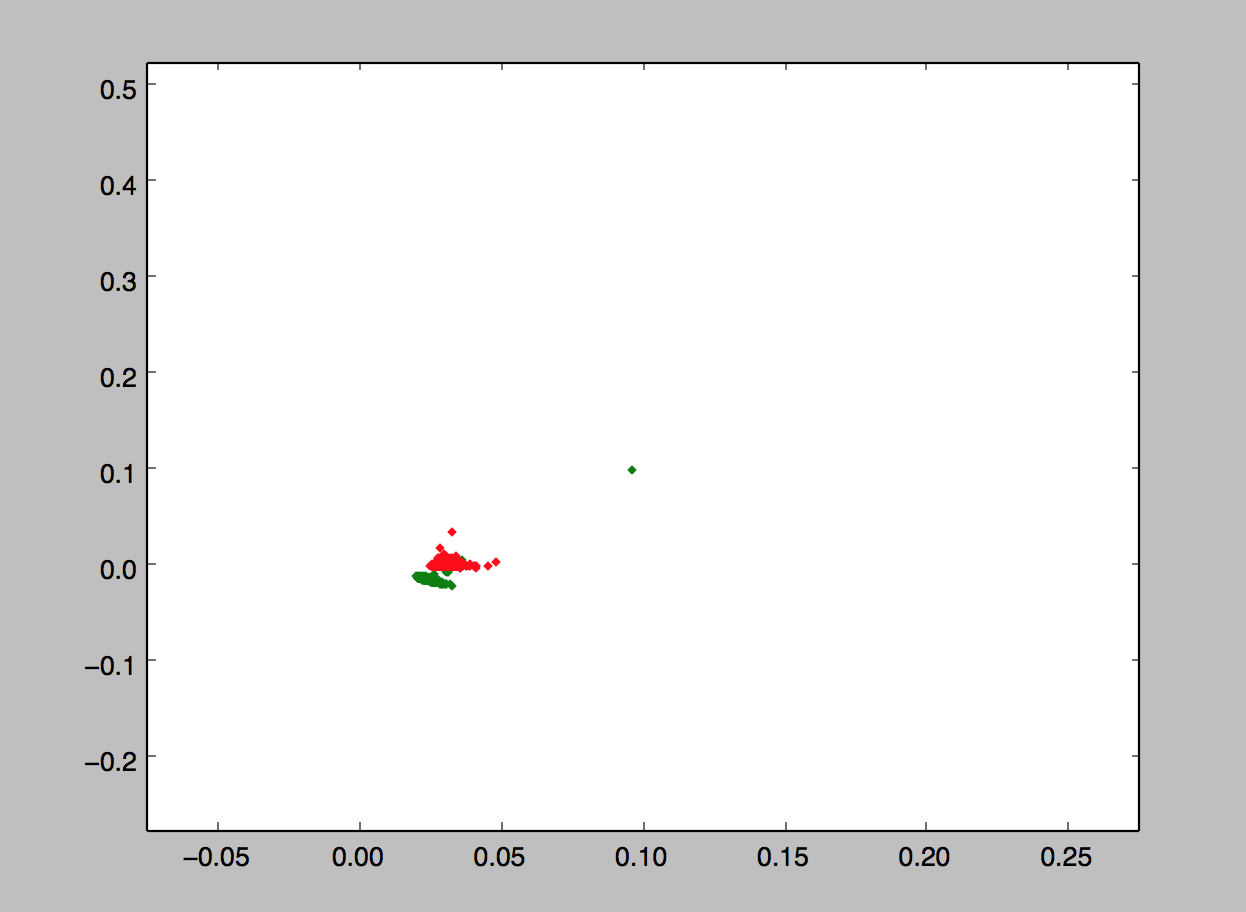
\includegraphics[width=5cm]{experiment_1} }}%
    \qquad
    \subfloat[LSA met term weighting]{{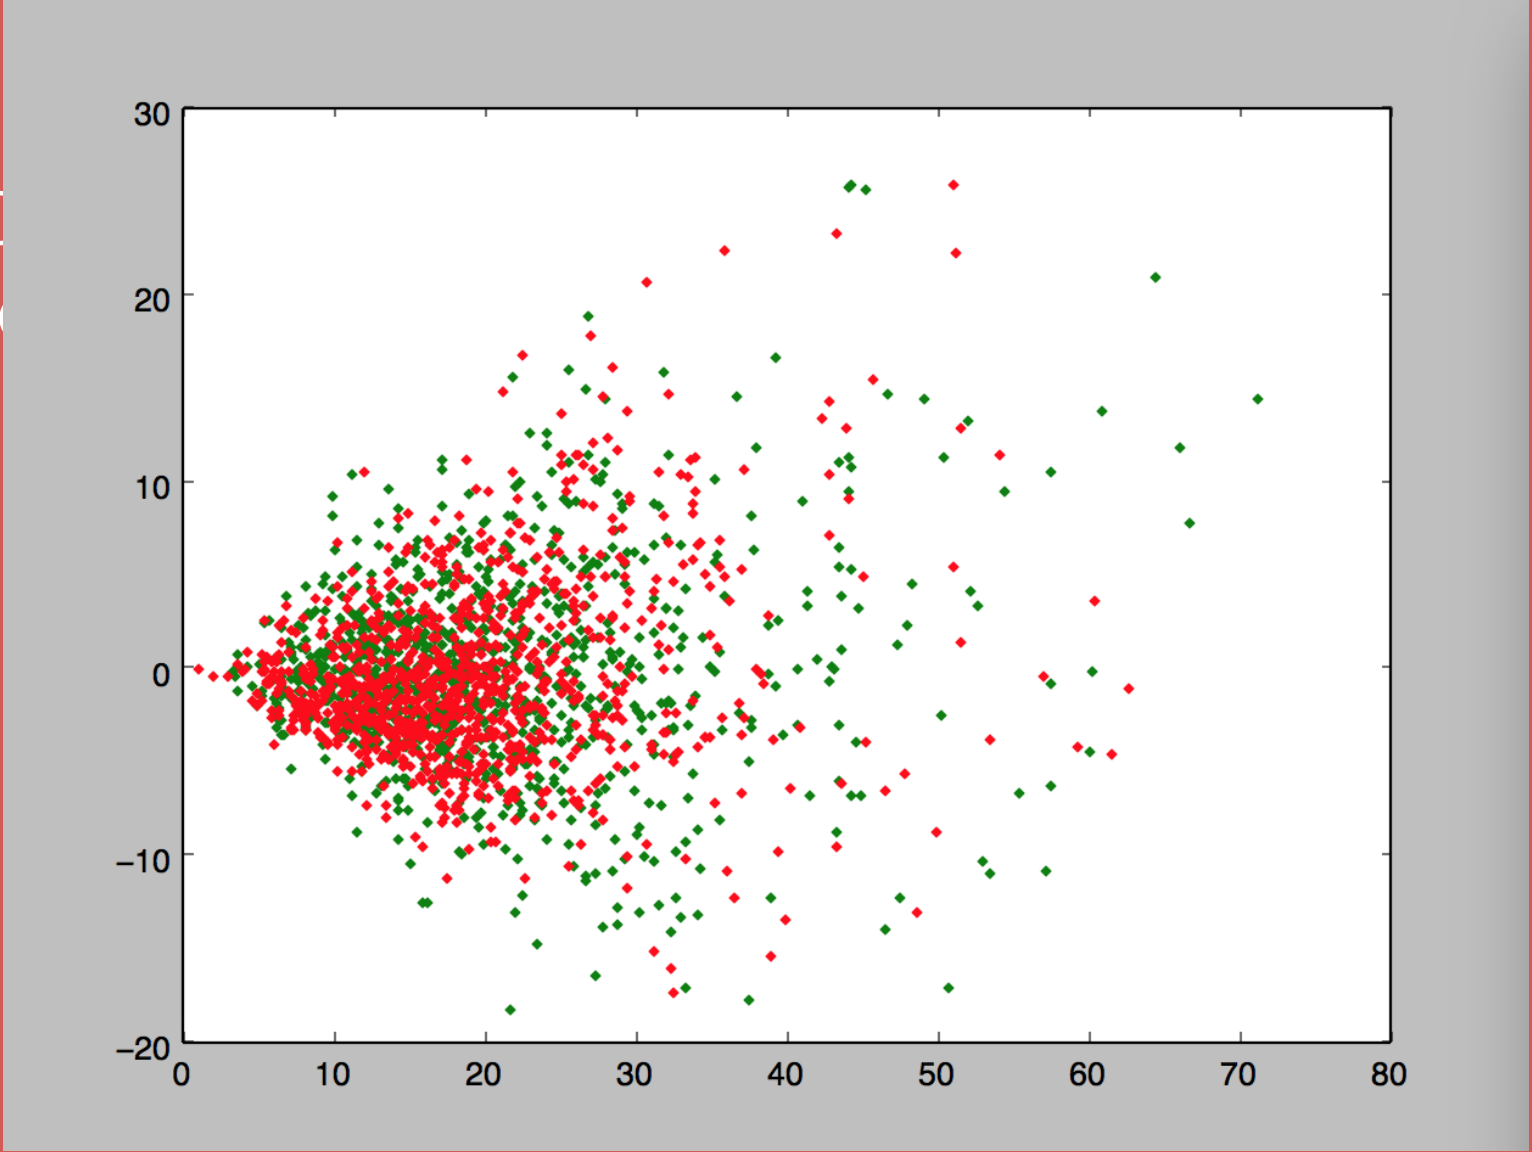
\includegraphics[width=5cm]{experiment_2} }}%
    \caption{Effect van term weighting voor LSA}%
    \label{fig:example}%
\end{figure}
%
Tenslotte kunnen we ook onze hypothese bevestigen. We zien dat de hoeveelheid aan features, de nauwkeurigheid van de classificatie beïnvloed. Onderstaande afbeelding geeft deze relatie weer. De x-waarde stelt het aantal gelijkaardige recensies dat men opvraagt voor. De y-waarde geeft aan hoeveel er gemiddeld effectief juist geclassifiseerd zijn. Belangrijk om te weten is dat de dataset voor de helft uit positieve recensies bestaat en voor de helft uit negatieve. We trachten dus bij de classificatie een gemiddeld percentage van 50 percent te halen en we zien dat op onderstaand voorbeeld de lijn van 500 features hier het beste in slaagt.


\begin{center}
  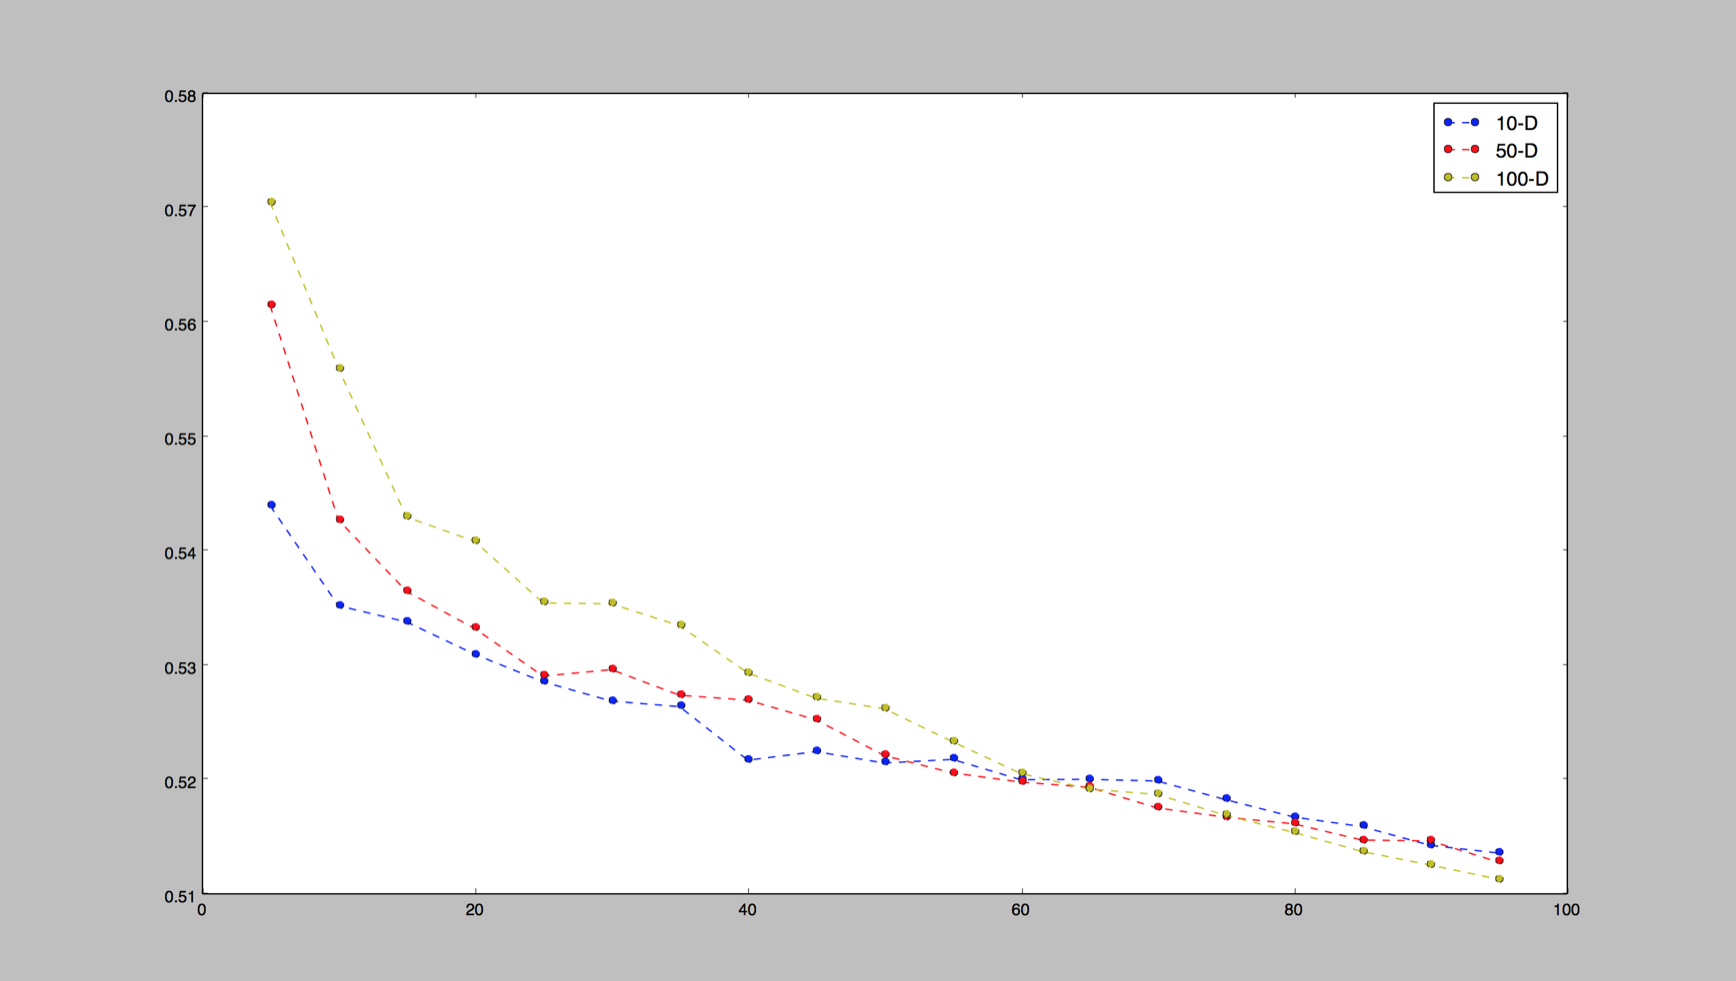
\includegraphics[width=10cm]{experiment_3}
  \captionof{figure}{Nauwkeurigheid van de classificatie bij een verschillend aantal features}
\end{center}
\endgroup
\chapter{Conclusie}\label{Conclusie}

Voor deze bachelorproef gingen we onderzoeken of de werkwijzen voor engelstalige gevoelsanalyse ook toepasbaar zijn voor nederlandstalige gevoelsanalyse en proberen we deze verschillen beter te specificeren. We hebben getracht om aan de hand van een experimentele analyse hier een antwoord op te vinden.
In de experimentele analyse hebben we een algemeen beeld proberen te vormen over Nederlandse gevoelsanalyse. We hebben in \ref{Engelse gevoelsanalyse versus Nederlandse Gevoelsanalyse} een directe vergelijking gemaakt met Engelse gevoelsanalyse. In deze vergelijking zagen we dat Engelse gevoelsanalyse in het algemeen beter presteerde dan Nederlandse gevoelsanalyse, maar dat voor beide gevoelsanalyses er goede resultaten werden behaald. En de technieken voor Engelse gevoelsanalyse wel degelijk overdraagbaar zijn naar Nederlandse gevoelsanalyse. We zijn mogelijke oorzaken van die betere prestatie voor het Engels gaan onderzoeken. Hieruit konden we besluiten dat de impact van de hoeveelheid woorden (data) in een tekst een rol spelen in de prestatie. We zagen een duidelijk prestatie voordeel bij de Engelse dataset met langere woorden. Dit bevestigd nogmaals dat een goed presterende gevoelsanalyse met de huidige technieken enkel mogelijk is voor meer substanti\"ele teksten, en moeilijk tot onmogelijk voor kortere stukken tekst.\\
Ook zagen we in beide analyseresultaten dezelfde trends. Zo zagen we voor beide talen de Naive Bayes Classifier in combinatie met het verwijderen van stopwoorden, Term weighting en Bigrams als beste techniek en zagen we dezelfde prestatieverschillen tussen de algoritmen mee overgaan van het Engels naar het Nederlands.\\

Vervolgens hebben we classificatie onderzocht op basis van geannoteerde woordenlijsten van gevoelens. Hier hadden we voor de Nederlandse woordenlijsten, een vertaling gebruikt van de Engelse woordenlijsten. Hier konden we besluiten dat Engels woordenlijsten niet transparant vertaald kunnen worden naar het Nederlands en de classificatie onvoldoende presteert. We zagen hier deels de oorzaak lag bij een andere woordenschat, leenwoorden, schrijffouten, internetslang en uitgesmeerde woorden. In verder onderzoek kan men deels deze invloeden wegnemen door de woordenlijsten zelf samen te stellen op basis van een Nederlandse dataset en hier de prestatie van te onderzoeken. Een andere opvallende bevinding uit dit experiment is de opvallende overeenkomst van negatieve engelstalige woorden in onze Nederlandse dataset. Dit kan ook een gevolg zijn van de herkomst van onze Nederlandse dataset (een ‘internetpubliek’ dat onder andere veel gebruikt maakt van anglicismen).\\

Als laatste hebben we de invloed van jargon onderzocht bij Nederlandse gevoelsanalyse. Hier zagen we dat wanneer men een classifier traint voor een bepaald jargon deze ook het beste presteert voor dat jargon. Ook zagen we dat een algemeen concept, het onderscheiden van een positieve en negatieve opinie, kan aangenomen worden door de classifier, desondanks het jargon in de datasets.\\

We hebben aangetoond dat technieken voor gevoelsanalyse grotendeels overdraagbaar zijn, al is het belangrijk om rekening te houden met het feit dat technieken die afhangen van uitgebreid geannoteerde woordenlijsten vaak niet rechtstreeks te vertalen zijn. Voor deze aanpakken is het dus nodig om per taal aangepaste woordenlijsten op te stellen. Maar gezien de goede prestaties van technieken die zonder deze lijsten kunnen werken, kunnen we stellen dat het vaak interessanter is om te investeren in de ontwikkeling van een goede herbruikbare leertechniek in plaats van een uitgebreide geannoteerde woordenlijst per taal.
\newpage
\nocite{*}
\bibliographystyle{apacite}
\bibliography{sections/Thesisbib}
\end{document}
    
    
        